% Copyright (C) 2014-2023 by Thomas Auzinger <thomas@auzinger.name>

% TODO: remove draft
\documentclass[draft,final]{vutinfth} % Remove option 'final' to obtain debug information.

% Load packages to allow in- and output of non-ASCII characters.
\usepackage{lmodern}        % Use an extension of the original Computer Modern font to minimize the use of bitmapped letters.
\usepackage[T1]{fontenc}    % Determines font encoding of the output. Font packages have to be included before this line.
\usepackage[utf8]{inputenc} % Determines encoding of the input. All input files have to use UTF8 encoding.

% Extended LaTeX functionality is enables by including packages with \usepackage{...}.
\usepackage{amsmath}    % Extended typesetting of mathematical expression.
\usepackage{amssymb}    % Provides a multitude of mathematical symbols.
\usepackage{mathtools}  % Further extensions of mathematical typesetting.
\usepackage{microtype}  % Small-scale typographic enhancements.
\usepackage[inline]{enumitem} % User control over the layout of lists (itemize, enumerate, description).
\usepackage{multirow}   % Allows table elements to span several rows.
\usepackage{booktabs}   % Improves the typesetting of tables.
\usepackage{subcaption} % Allows the use of subfigures and enables their referencing.
\usepackage[ruled,linesnumbered,algochapter]{algorithm2e} % Enables the writing of pseudo code.
\usepackage[usenames,dvipsnames,table]{xcolor} % Allows the definition and use of colors. This package has to be included before tikz.
\usepackage{nag}       % Issues warnings when best practices in writing LaTeX documents are violated.
\usepackage{todonotes} % Provides tooltip-like todo notes.
\usepackage{hyperref}  % Enables hyperlinking in the electronic document version. This package has to be included second to last.
\usepackage[acronym,toc]{glossaries} % Enables the generation of glossaries and lists of acronyms. This package has to be included last.

% custom packages
\usepackage{threeparttable}
\usepackage{makecell}
\usepackage{tikz}
\usetikzlibrary{arrows.meta}


% Define convenience functions to use the author name and the thesis title in the PDF document properties.
\newcommand{\authorname}{Othmar Lechner} % The author name without titles.
\newcommand{\thesistitle}{T-RACE: Tracing race condition attacks between Ethereum transactions.} % The title of the thesis. The English version should be used, if it exists.

% Set PDF document properties
\hypersetup{
    pdfpagelayout   = TwoPageRight,           % How the document is shown in PDF viewers (optional).
    linkbordercolor = {Melon},                % The color of the borders of boxes around hyperlinks (optional).
    pdfauthor       = {\authorname},          % The author's name in the document properties (optional).
    pdftitle        = {\thesistitle},         % The document's title in the document properties (optional).
    pdfsubject      = {Subject},              % The document's subject in the document properties (optional).
    pdfkeywords     = {a, list, of, keywords} % The document's keywords in the document properties (optional).
}

\setpnumwidth{2.5em}        % Avoid overfull hboxes in the table of contents (see memoir manual).
\setsecnumdepth{subsection} % Enumerate subsections.

\nonzeroparskip             % Create space between paragraphs (optional).
\setlength{\parindent}{0pt} % Remove paragraph indentation (optional).

\makeindex      % Use an optional index.
\makeglossaries % Use an optional glossary.
%\glstocfalse   % Remove the glossaries from the table of contents.

% Set persons with 4 arguments:
%  {title before name}{name}{title after name}{gender}
%  where both titles are optional (i.e. can be given as empty brackets {}).
\setauthor{}{\authorname}{}{male}
\setadvisor{Pretitle}{Forename Surname}{Posttitle}{male}

% For bachelor and master theses:
\setfirstassistant{Pretitle}{Forename Surname}{Posttitle}{male}
\setsecondassistant{Pretitle}{Forename Surname}{Posttitle}{male}
\setthirdassistant{Pretitle}{Forename Surname}{Posttitle}{male}

% For dissertations:
\setfirstreviewer{Pretitle}{Forename Surname}{Posttitle}{male}
\setsecondreviewer{Pretitle}{Forename Surname}{Posttitle}{male}

% For dissertations at the PhD School and optionally for dissertations:
\setsecondadvisor{Pretitle}{Forename Surname}{Posttitle}{male} % Comment to remove.

% Required data.
\setregnumber{11841833}
\setdate{01}{01}{2001} % Set date with 3 arguments: {day}{month}{year}.
\settitle{\thesistitle}{T-RACE: Eine Analyse von race condition Angriffen bei Ethereum Transaktionen} % Sets English and German version of the title (both can be English or German). If your title contains commas, enclose it with additional curvy brackets (i.e., {{your title}}) or define it as a macro as done with \thesistitle.
% \setsubtitle{Optional Subtitle of the Thesis}{Optionaler Untertitel der Arbeit} % Sets English and German version of the subtitle (both can be English or German).

% Select the thesis type: bachelor / master / doctor.
% Bachelor:
% \setthesis{bachelor}
%
% Master:
\setthesis{master}
% TODO: dipl. or master?
\setmasterdegree{dipl.} % dipl. / rer.nat. / rer.soc.oec. / master
%
% Doctor:
%\setthesis{doctor}
%\setdoctordegree{rer.soc.oec.}% rer.nat. / techn. / rer.soc.oec.

% For bachelor and master:
\setcurriculum{Software Engineering \& Internet Computing}{Software Engineering \& Internet Computing} % Sets the English and German name of the curriculum.

% Optional reviewer data:
\setfirstreviewerdata{Affiliation, Country}
\setsecondreviewerdata{Affiliation, Country}


\begin{document}

\frontmatter % Switches to roman numbering.
% The structure of the thesis has to conform to the guidelines at
%  https://informatics.tuwien.ac.at/study-services

\addtitlepage{naustrian} % German title page.
\addtitlepage{english} % English title page.
\addstatementpage

\begin{danksagung*}
    \todo{Ihr Text hier.}
\end{danksagung*}

\begin{acknowledgements*}
    \todo{Enter your text here.}
\end{acknowledgements*}

\begin{kurzfassung}
    \todo{Ihr Text hier.}
\end{kurzfassung}

\begin{abstract}
    \todo{Enter your text here.}
\end{abstract}

% Select the language of the thesis, e.g., english or naustrian.
\selectlanguage{english}

% Add a table of contents (toc).
\tableofcontents % Starred version, i.e., \tableofcontents*, removes the self-entry.

% Switch to arabic numbering and start the enumeration of chapters in the table of content.
\mainmatter

\chapter{Introduction}
\todo{Enter your text here.}

\section{Related work}

Interesting things:
- name
- source is available?
- does it use RPC / instrumentation / native tracing?
- does it detect some kind of frontrunning

See table \ref{tab:blockchain_history_analyzers}.


% TODO: is there related work in the parallel EVM field? TOD is highly relevant for this
% https://ieeexplore.ieee.org/abstract/document/10102454


\begin{table}[h]
    \begin{center}
        \begin{tabular}{ | l | c  | c | c | c | }
            \hline
            Tool/Authors                                     & Scope            \\ \hline
            EthScope \cite{wu_time-travel_2022}              & Generalized      \\ \hline
            TokenScope \cite{chen_tokenscope_2019}           & ERC-20 tokens    \\ \hline
            TXSPECTOR \cite{zhang_txspector_2020}            & Generalized      \\ \hline
            Horus \cite{ferreira_torres_eye_2021}            & Generalized      \\ \hline
            SODA \cite{chen_soda_2020}                       & Generalized      \\ \hline
            DEFIER \cite{su_evil_2021}                       & Generalized      \\ \hline
            Zhou et al. \cite{zhou_ever-evolving_2020}       & Generalized      \\ \hline
            Perez et al. \cite{perez_smart_2021}             & Generalized      \\ \hline
            Wang et al. \cite{wang_impact_2022}              & Sandwich attacks \\ \hline
            Erebus-redgiant \cite{zhang_combatting_2023}     & Frontrunning     \\ \hline
            Frontrunner Jones \cite{torres_frontrunner_2021} & Frontrunning     \\ \hline
        \end{tabular}
        \caption{Blockchain history analysis references. Generalized means, that the data collection and analysis framework is not tailored to specific vulnerabilities.}
        \label{tab:blockchain_history_analyzers}
    \end{center}
\end{table}
\todo{Better caption}

\section{Related approaches}

\subsection{Combatting paper - Erebus-redgiant}

How do they replay potential attack/victim transactions?

Their framework allows forking at a specific block and tx index.

PrepareStateAndContext - replays up to tx index.


They skip potential victim transactions if:

\begin{enumerate}
    \item error victim transactions (\todo{Are these failed transactions in Ethereum, or error somewhere in their framework? If it's the first, why???})
    \item "filtered" transactions \todo{What are these?}
    \item unverified contracts in victim transactions
    \item victim tx is contract creation (why???). But a good label :)
    \item victim tx is ether transfer
    \item no overlap with attack tx (compare sets of contracts/accounts)
    \item no dependency (storage and balance dependencies, but seem to ignore dependencies within reverted calls)
\end{enumerate}

Replaying in the attack free scenario:

\begin{enumerate}
    \item take attack tx state (I guess prestate)
    \item take victim context (I guess block environment, timestamp, ...)
    \item apply "prerequesites" - all previous transactions from the same sender within (attack, victim-1)?
    \item apply + trace victim tx
    \item apply + trace attack tx
\end{enumerate}

For prerequisites, refer to \href{https://github.com/Troublor/erebus-redgiant/blob/4544163f0c6a369b35c3237851f482d240fa7bbd/dataset/tx_history_test.go#L42-L53}.

Problems with this approach:

\begin{enumerate}
    \item Prerequisites is an arbitrary choice
          \subitem what if prerequisites have collisions with the attack?
          \subitem what if prerequisites depend on other transactions that were not replayed?
          \subitem what if victim tx depends on other transactions that were not replayed?
    \item all transactions share the same context
          \subitem attack tx is moved to different context
          \subitem prerequisites are potentially moved to different context
          \subitem (victim tx stays in same context \checkmark)
    \item replay is done with a different environment
\end{enumerate}

\chapter{Background}

This chapter gives background knowledge on Ethereum, that is helpful to follow the remaining paper.

\section{Ethereum}

Ethereum is a blockchain, that can be characterized as a "transactional singleton machine with shared-state" \cite{wood_ethereum_2024}. By using a consensus protocol, a decentralized set of nodes agrees on a globally shared state. This state contains two types of accounts: \emph{externally owned accounts} (EOA) and \emph{contract accounts} (also referred to as smart contracts). Each account is identified by a 20 byte address. The shared state is modified by executing \emph{transactions} \cite{tikhomirov_ethereum_2018}.

\section{World State}

Similar to \cite{wood_ethereum_2024}, we will refer to the shared state as \emph{world state}. The world state maps addresses to account states, containing a \emph{nonce}, \emph{balance}, \emph{storage} and \emph{code}\footnote{Technically, the account state only contains hashes that identify the storage and code, not the actual storage and code. This distinction is not relevant in this paper.}. They store following data \cite{wood_ethereum_2024}:

\begin{itemize}
    \item \emph{nonce}: For EOAs, this is the number of transactions submitted by this account. For contract accounts, this is the number of contracts created by this account.
    \item \emph{balance}: The value of Wei, a smaller unit of Ether.
    \item \emph{storage}: For contract accounts, the storage a mapping of storage slots to values. Both, key and value, are 256 bytes. For EOAs, this is empty.
    \item \emph{code}: For contract accounts, the code is a sequence of EVM instructions.
\end{itemize}

We denote the world state as $\sigma$, the account state of an address $a$ as $\sigma(a)$ and the nonce, balance, storage and code as $\sigma(a)_n$, $\sigma(a)_b$, $\sigma(a)_s$ and $\sigma(a)_c$ respectively.

\section{EVM}

The Ethereum Virtual Machine (EVM) is used to execute code in Ethereum. It can execute a set of instructions, that can access and modify the world state. The EVM is Turing-complete, except that it is executed with a limited amount of \emph{gas} and each instruction costs some gas \cite{wood_ethereum_2024}. When it runs out of gas, the execution will halt \cite[p.14]{wood_ethereum_2024}. For instance, this prevents execution of infinite loops, as it would use infinitely much gas and thus exceed the gas limit.

Most EVM instructions are formally defined in \cite[p.30-38]{wood_ethereum_2024}. However, the Yellowpaper currently does not include the changes from the Cancun upgrade \cite{noauthor_history_2024}, therefore we will also refer to the informal description available on \href{https://www.evm.codes/}{evm.codes} \cite{noauthor_evm_2024}.

\section{Transactions}

A transaction can modify the world state by transferring Ether and executing EVM code. It must be signed by the owner of an EOA and contains following data relevant to our work:

\begin{itemize}
    \item \emph{sender}: The address of the transaction sender\footnote{The sender is only implicitly given through the signature and the transaction hash \cite[p.25-27]{wood_ethereum_2024}. We are only interested in transactions that are included in the blockchain, thus the signature must be valid and the transaction's sender can always be computed.}.
    \item \emph{recipient}: The destination address.
    \item \emph{value}: The value of Wei that should be transferred from the sender to the recipient.
    \item \emph{gasLimit}: The maximum number of gas, that can be used for the execution.
\end{itemize}

If the recipient address is empty, the transaction will create a new contract account. These transactions also include an \emph{init} field, that contains the code to initialize the new contract account.

When the recipient address is given, the value will be transferred to the recipient and, if the recipient is a contract account, also execute the recipient's code. The transaction can specify a \emph{data} field to pass input data to the code execution \cite[p.4-5]{wood_ethereum_2024}.

% TODO: move \cite to pre/post period.

For every transaction the sender must pay a \emph{transaction fee}. This is composed of a \emph{base fee} and a \emph{priority fee}. Every transaction must pay the base fee. The amount of Wei will be reduced from the sender and not given to any other account. For the priority fee, the transaction can specify if, and how much they are willing to pay. This fee will be taken from the sender and given to the block validator, explained in the next section \cite[p.8]{wood_ethereum_2024}.

We denote a transaction as $T$, sometimes adding a subscript $T_A$ to differentiate from another transaction $T_B$.

% TODO: rename block producer to block validator

\section{Blocks}

The Ethereum blockchain consists of a sequence of blocks, where each block builds upon the state of the previous block. To achieve consensus about the canonical sequence of blocks in a decentralized network of nodes, Ethereum currently uses a consensus protocol. In this protocol, validators build and propose blocks to be added to the blockchain \cite{noauthor_gasper_2024}. It is the choice of the validator, which transactions to include in a block, however they are incentivized to include transactions that pay high transaction fees, as they receive the fee \cite[p.8]{wood_ethereum_2024}.

Each block consists of a block header and a sequence of transactions. We denote the nth block of the blockchain as $B_n$ and the sequence of transactions it includes as $T(B_n) = (T_1, T_2, \dots, T_m)$.

\section{Transaction submission}

This section discusses, how a signed transaction by an EOA ends up being included in the blockchain.

Traditionally, the signed transaction is broadcasted to the network of nodes, which temporarily store them in a \emph{mempool}, a collection of pending transactions. The creator of the next block then picks transactions from the mempool and includes them in the next block \cite{eskandari_sok_2020}. In this submission method, the pending transactions in the mempool are publicly known to the nodes in the network, even before being included in the blockchain. This time window will be important for our discussion on frontrunning, as it gives nodes time to react on a transaction before it is executed on the blockchain.

A different approach, the Proposer-Builder Separation (PBS) has become more popularity recently: Here, we separate the task of collecting transactions and building blocks with them from the task of proposing them as a validator \cite{heimbach_ethereums_2023}. A user submits their signed transaction or transaction bundle to a block builder. The block builder has a private mempool and uses it to create profitable blocks. Finally, the validator picks one of the created blocks and adds it to the blockchain.

\section{Nodes}

A node consists of an \emph{execution client} and a \emph{consensus client}. The execution client keeps track of the world state and the mempool and executes transactions. The consensus client takes part in the consensus protocol. For this work, we will use an \emph{archive node}, which is a node that allows to reproduce the state and transactions at any block \cite{noauthor_nodes_2024}.

\section{RPC}

Execution clients implement the Ethereum JSON-RPC specification \cite{noauthor_ethereum_2024}. It provides an API to access the execution client, for instance to inspect the current block number with \verb|eth_blockNumber| or to execute a transaction without committing the state via \verb|eth_call|. In addition to the standardized RPC methods, we will also make use of methods in the debug namespace, such as \verb|debug_traceBlockByNumber|. While this namespace is not standardized, several execution clients implement these additional methods \cite{noauthor_debug_2024}\cite{noauthor_rpc_2024}\cite{noauthor_reth_2024}.


\chapter{TOD and Frontrunning definitions}

\section{Transaction execution}

In Ethereum, transaction execution is deterministic: If the transaction is executed in a specific block environment and world state, it will always produce the same result. The result is used to update the world state, which we model as a function $\Pi(T, E, \sigma) = \sigma\prime$, where $T$ is the transaction, $E$ is the block environment and $\sigma$ is the world state.

In this paper, we are interested in the effects of the transaction order. If we reorder transactions across multiple blocks, they would execute in a different block environment than they did originally. The effects of block environments are already covered in several other vulnerability definitions\todo{Reference}. Thus, we will exclude the possibility of changing block environments and assume that transactions are always executed in their original block environment. As such, we can think of the transaction execution as $\Pi(T, \sigma) = \sigma\prime$, also denoted as $\sigma \xrightarrow{T} \sigma\prime$ in the following.

\todo{Notation for multiple transactions}

\section{Transaction order dependence}

We say, that a pair of transactions $(T_A, T_B)$ is transaction order dependent (TOD), if and only if:

$$\sigma \xrightarrow{T_A, T_B} \sigma \prime$$
$$\sigma \xrightarrow{T_B, T_A} \sigma \prime \prime$$
$$\sigma \prime \neq \sigma \prime \prime$$

\todo{What about logs? These are not part of the world state, but should also be modelled.}

\subsection{Collision}

Transactions are influenced by the world state and can also modify it. When a transaction $T$ accesses the world state, we denote it as $R_T$, when it modifies the world state, we denote it as $W_T$.

$$R_T = \{ balance(addr), code(addr), nonce(addr), storage(addr, key) \}$$
$$W_T = \{ balance(addr), code(addr), nonce(addr), storage(addr, key) \}$$

We define the state collisions of two transactions as:

$$collisions(T_A, T_B) = (W_{T_A} \cap R_{T_B}) \cup (W_{T_A} \cap W_{T_B})$$ \todo{Do I want read-write as well? Would be TOD, but not an attack.}

With $W_{T_A} \cap R_{T_B}$ we include write-read collisions, where $T_A$ modifies some state and $T_B$ accesses the same state. Therefore, the execution of $T_B$ depends on the value that $T_A$ wrote, which is a potential TOD. With $W_{T_A} \cap W_{T_B}$ we include write-write collisions, where both transactions write to the same state location. In this case, the value of this state location depends on which transaction was executed last, and thus this also is a potential TOD.

\subsection{TOD candidate}

We will refer to a transaction pair $(T_A, T_B)$, where $T_A$ was executed before $T_B$ and $collisions(T_A, T_B) \neq \emptyset$ as a TOD candidate.

A TOD candidate is not necessarily TOD, for instance consider the case that $T_B$ only reads the value that $T_A$ wrote but never uses it for any computation. This would be a TOD candidate, as they have a collision, however the result of executing $T_B$ is not impacted by this collision.

\todo{Write somewhere that being a TOD candidate is necessary for TOD.}

\subsection{State accessing instructions}

The EVM instructions in table \ref{tab:state_reading_instructions} can access the world state. For most the reason of the access is clear, for instance \verb|BALANCE| needs to access the balance of the target address.
\todo{Write that I got this from the wood paper.}

Less obvious is the nonce access of several instructions, which is because the EVM uses the nonce (among other things) to check if an account already exists. For CALL, CALLCODE and SELFDESTRUCT, this is used to calculate the gas costs. For CREATE and CREATE2, this is used to prevent creating an account at an already active address. \cite{wood_ethereum_2024}

\begin{table}[h]
    \begin{center}
        \begin{tabular}{ | l | c  | c | c | c | }
            \hline
            Instruction  & Storage    & Balance    & Code       & Nonce      \\ \hline
            SLOAD        & \checkmark &            &            &            \\ \hline
            BALANCE      &            & \checkmark &            &            \\ \hline
            SELFBALANCE  &            & \checkmark &            &            \\ \hline
            CODESIZE     &            &            & \checkmark &            \\ \hline
            CODECOPY     &            &            & \checkmark &            \\ \hline
            EXTCODECOPY  &            &            & \checkmark &            \\ \hline
            EXTCODESIZE  &            &            & \checkmark &            \\ \hline
            EXTCODEHASH  &            &            & \checkmark &            \\ \hline
            CALL         &            & \checkmark & \checkmark & \checkmark \\ \hline
            CALLCODE     &            & \checkmark & \checkmark & \checkmark \\ \hline
            STATICCALL   &            &            & \checkmark &            \\ \hline
            DELEGATECALL &            &            & \checkmark &            \\ \hline
            CREATE       &            & \checkmark & \checkmark & \checkmark \\ \hline
            CREATE2      &            & \checkmark & \checkmark & \checkmark \\ \hline
            SELFDESTRUCT &            & \checkmark & \checkmark & \checkmark \\ \hline
        \end{tabular}
        \caption{Instructions that access state. A checkmark indicates, that the execution of this instruction can depend on this state type.}
        \label{tab:state_reading_instructions}
    \end{center}
\end{table}

\subsection{State modifying instructions}

In table \ref{tab:state_writing_instructions} we see instructions that can modify the world state.

\begin{table}[h]
    \begin{center}
        \begin{tabular}{ | l | c  | c | c | c | }
            \hline
            Instruction  & Storage    & Balance    & Code       & Nonce      \\ \hline
            SSTORE       & \checkmark &            &            &            \\ \hline
            CALL         &            & \checkmark &            &            \\ \hline
            CALLCODE     &            & \checkmark &            &            \\ \hline
            CREATE       &            & \checkmark & \checkmark & \checkmark \\ \hline
            CREATE2      &            & \checkmark & \checkmark & \checkmark \\ \hline
            SELFDESTRUCT & \checkmark & \checkmark & \checkmark & \checkmark \\ \hline
        \end{tabular}
        \caption{Instructions that modify state. A checkmark indicates, that the execution of this instruction can modify this state type.}
        \label{tab:state_writing_instructions}
    \end{center}
\end{table}

\section{todo}

\todo{Is it important to differentiate between sandwich attacks and displacement attacks?}
\todo{Should we go from first source to last sink? e.g. in a swap call, we will have multiple LOG events at different levels.}

\section{TOD sources}

For $T_A \rightarrow T_B$:

\todo{I think this is similar to the $attack altered data$ / taint source from the combatting paper}

\begin{enumerate}
    \item TOD write point: point, where $T_A$ modifies some state, that is read by $T_B$
    \item TOD read point: point, where $T_B$ reads some state, that was modified by $T_A$
    \item TOD hidden write point: point, where $T_A$ modifies some state, that is overwritten by $T_B$
    \item TOD overwrite point: point, where $T_B$ overwrites some state, that was written by $T_A$
\end{enumerate}

The pair of (TOD write point, TOD read point) presents a write-read conflict. The pair of (TOD hidden write point, TOD overwrite point) presents a write-write conflict.

If we have a write-read conflict and a write-write conflict, $T_B$ reads some state and then overwrites it. Thus, $T_B$ knows of the modified state before overwriting.

One instance would be a simple counter, where both $T_A$ and $T_B$ increment the same counter in the state. Here, we would have a write-read conflict, as $T_B$ reads the counter incremented by $T_A$. And further, we would have a write-write conflict, as $T_B$ updates the same counter as $T_A$.

ERC-20 approval attack would consist of the hidden write point (where approval is set to 0) and an overwrite point (where approval is set to some higher value).

ERC-20 approval mitigation (with require for the previous value) would consist of a write point (where approval is set to 0) and a read point (where the approval is used for the require statement).

Uniswap token swap would consist of both a write-read conflict and a write-write conflict. The write-read conflict exists, as $T_A$ modifies the reserves state and $T_B$ reads the current reserves to calculate a price. The write-write conflict exists, as $T_A$ modifies the reserves state and $T_B$ modifies it as well. Contrary to ERC-20 approval, the overwritten value depends on the previous value (which we could show in the data flow graph).

\section{TOD sinks}

\section{TOD sanitizers}

\chapter{TOD candidate mining}

In this chapter, we discuss how we search for potential TODs in the Ethereum history. The methodology is visualized in \todo{graph}. First, we use the \verb|debug_traceBlockByNumber| RPC method to obtain the accessed and modified state of the transactions and store them locally in a database. Then, we match the accessed and modified states of all transactions to get TOD transaction pairs, where one transaction modifies some state and the other transaction reads this state. For simplicity, we will call these potential TOD transaction pairs "TOD candidates". Finally, we use several heuristics to filter out TOD candidates, which are not relevant for the further analysis.

% NOTE: the mined attacks won't be representative of all contracts
%'s favored towards attacked contracts, and to frequently-used contracts

\section{TOD candidate finding}

In this step, we find transaction pairs $(T_A, T_B)$, such that $T_B$ read or modified some state, that was previously written by $T_A$. We consider all possible state modifications, namely nonce, balance, storage and code modifications.

For all blocks we analyze, we replay each transaction in this block with the \verb|debug_traceBlockByNumber| RPC method. Using the \verb|prestateTracer| we get the accessed state and state modifications by each transaction\footnote{When running the prestateTracer in diffMode, several fields are only implicit in the response. We need to make these fields explicit for further analysis. Refer to the documentation or the source code for further details.}\todo{reference}. We store this data in a local database for further analysis.

For a state access we store a $(T, K, V)$ entry, where $T$ is the state type, $K$ describes which state was accessed and $V$ is the accessed value. For instance, when a transaction reads the balance of a contract, we have $T = balance$, $K$ is the address of the contract and $V$ is the balance at this time. For nonce, balance and code we use the address as a key, and for storage slots we use the tuple of address and slot as a key.

For a state modification we store a $(T, K, V_{pre}, V_{post})$ entry. $T$ and $K$ are the same as before. $V_{pre}$ is the state value before execution of the transaction and $V_{post}$ the value after the execution.

After replaying all transactions, we match the state modifications with the state accesses. We query the database for transaction pairs $(T_A, T_B)$, where $T_A$ occurred before $T_B$ and $T_A$ has a state modification $(T, K, V_{pre}, V_{post})$ that matches a state access $(T, K, V_{post})$ of $T_B$.\todo{Reference indirect dependency section, add statistic what it would be without this}


\iffalse
    Contrary to the definition of TOD, this does not necessarily mean, that the execution of $T_B$ yields a different result because of $T_A$. For instance if $T_A$ modifies storage value from $1$ to $2$ and $T_B$ loads this storage value without using it, there is no impact on $T_B$. \todo{this should go to the definition/general TOD discussion section}
\fi




\begin{figure}[h]
    \centering
    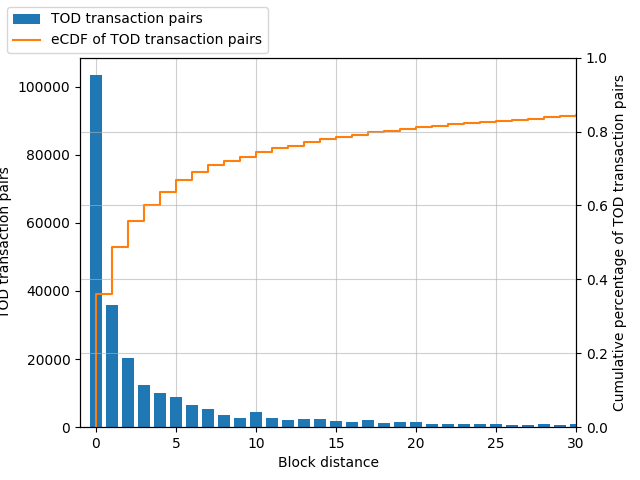
\includegraphics[width=0.8\textwidth]{tod_collisions_hist.png}
    \caption{The histogram and eCDF of the block distance for TOD transaction pairs. The blue bars show how many TOD transaction pairs have been found that are n blocks apart. The orange line shows the percentage of TOD transaction pairs, that are at most n blocks apart.}
    \label{fig:tod_block_dist}
\end{figure}


\section{TOD candidate filtering}

Many of the TOD candidates we gain in the previous section are not relevant for our further analysis. To prevent unnecessary computation and distortion of our results, we filter them out.

\begin{table}[h]
    \begin{center}
        \begin{tabular}{ | l | l |  }
            \hline
            \thead{Filter name}      & \thead{Short description}                                  \\ \hline
            Indirect dependency      & \makecell[l]{$T_A$ could indirectly influence $T_B$.       \\For instance, if candidates $(T_A, T_X)$ and $(T_X, T_B)$ exist.} \\ \hline
            Block producers          & The state overlap is only the balance of a block producer. \\ \hline
            EOA nonce                & The state overlap is only the nonce of an EOA.             \\ \hline
            Same sender              & $T_A$ is from the same sender as $T_B$.                    \\ \hline
            Recipient Ether transfer & $T_B$ is an Ether transfer without code execution.         \\ \hline
            % Maybe: what else?
        \end{tabular}
        \caption{TOD candidate filters.}
        \label{tab:tod_candidate_filters}
    \end{center}
\end{table}

We filter a TOD candidate $(T_A, T_B)$ if any of the filters from table \ref{tab:tod_candidate_filters} applies. The filters are explained in the following section.

\subsection{Filters}

\subsubsection{Block producers}

In Ethereum, each transaction must pay a transaction fee to the block producer and thus modifies the block producer's\todo{Is this a correct '?} balance. This would qualify each transaction pair in a block as a TOD candidate, as they all modify the balance of the block producer's address.

We exclude TOD candidates, where the only collision\todo{Did we define "collision" previously?} is the balance of any block producer.

\todo{Graph on transaction fee dependencies}

\subsubsection{Indirect dependency}

\iffalse
    The overall goal of our analysis, is to analyze the effects of the transaction order. For this, we will take a TOD candidate $(T_A, T_B)$ and analyze what would have happened if they were executed in the opposite order, i.e. $(T_B, T_A)$.
\fi

As argued in section \todo{x}, indirect dependencies can hinder our analysis. We already have a model of all direct (potential) dependencies with the TOD candidates. We can build a transaction dependency graph $G = (V, E)$ with $V$ being all transactions and $E = \{ (T_A, T_B) \mid (T_A, T_B) \in \text{TOD candidates} \}$. We then filter out all TOD candidates $(T_A, T_B)$ where there exists a path $T_A, T_{X_1}, \dots, T_{X_n}, T_B$ with at least one intermediary node $T_{X_i}$.

Figure \ref{fig:tod_candidate_dependency} shows an example dependency graph, where transaction $A$ influences both $X$ and $B$ and $B$ is influenced by all other transactions. We would filter out the candidate $(A, B)$ as there is a path going over $X$, but keep $(X, B)$ and $(C, B)$.

For soundness, we would want to apply this filter first: If another filter removes a TOD candidate, the information about this dependency is removed from the dependency graph, and we could miss potential indirect dependencies. However, because of transaction fees, there would be a dependency between every transaction of the same block, and we have an indirect dependency between nearly all transactions of a block. This dependency could only be a problem, if a transaction actually uses the balance value of the miner. We neglect this case, and filter out block producer dependencies first.

\begin{figure}[h]
    \centering
    \begin{tikzpicture}
        \begin{scope}[
            >={Stealth[black]},
            every node/.style={circle,thick,draw},
            every edge/.style={draw=red,very thick}
            ]
            \node (A) at (3, 6) {A};
            \node (B) at (4, 3) {B};
            \node (C) at (5, 5) {C};
            \node (X) at (2, 4) {X};
            \path [->] (A) edge (B);
            \path [->] (A) edge (X);
            \path [->] (X) edge (B);
            \path [->] (C) edge (B);
        \end{scope}
    \end{tikzpicture}
    \caption{TOD candidate filters.}
    \label{fig:tod_candidate_dependency}
\end{figure}

\subsubsection{Same sender}

If the sender of both transactions is the same, they would have attacked themselves.

To remove these TOD candidates, we use the information from the \verb|eth_getBlockByNumber| RPC method and compare the sender fields for $T_A$ and $T_B$.

\subsubsection{EOA nonce}

% TODO: not exactly true / not argued well enough. What if 2nd transaction accesses EOA nonce? I guess not possible, be explicit about that

The nonce of an externally owned account is only increased when they send a transaction. As such, a collision on EOA nonces can only occur if both transactions are from the same sender. However, when using the state accesses and modifications from \verb|debug_traceBlockByNumber|, it also marks the nonce of EOA accounts as accessed, even if only the balance was accessed.

To exclude these cases, where the nonce is wrongly included in the accessed fields, we remove nonce accesses for EOA addresses.

\subsubsection{Recipient Ether transfer}

If a transaction sends Ether without execution code, it only depends on the balance of the EOA that signed the transaction. Other entities could only increase the balance of this EOA, by frontrunning the transaction, which has no adverse effects on the transaction.

When a transaction executes code, the trace will show this code access. Thus, we can exclude TOD candidates, where $T_B$ has no code access.

% TODO: extend this also to sender ether transfers. It's probably the same argument
% The receiver of an eth transfer without code exection must be EOA
% However, the 2nd transaction *could* read the balance of this EOA
% and thus be impacted by the 1st transfer -> could filter with an opcode tracer

\subsection{Deduplication}

We want a diverse set of attacks for the benchmark, so we filter out similar attacks to the ones we already analyzed. For instance, it does not make sense to analyze 5000 attacks for the USDT Stablecoin, as these will mostly collide.

If possible, we don't need the traces analyzer for deduplication. For instance, maybe we can get all the necessary information from the default RPC tracers.
Alternatively, we could also download all necessary data, and then loop through the traces analyzer and only pick the relevant (deduplicated) potential attacks.

Ideas, potentially a mixture of those:

\begin{enumerate}
    \item only trace some attacks per contract
    \item only trace some attacks per function
    \item only trace some attacks per group of vulnerable contracts (as defined by analysis)
    \item only trace some attacks per contract/function skeletons
    \item similar to \cite{}, analyze at how many attacks per contract/function the number of found attacks saturate (based on the analysis result)
\end{enumerate}

\chapter{Trace analysis}

% For instance, all EVM transactions in the same block read and write to the beneficiary account for gas payment, making all transactions interdependent by default.
% Is this the case? Do we see this in the prestate tracer?
% https://github.com/risechain/pevm

\section{Trace replaying}

\subsection{RPC methods}


\todo{\href{https://github.com/paradigmxyz/reth/issues/8202}{Prestate tracer currently does not include prestate for reverted call contexts}}
\todo{Use quicknode RPC to compare stateDiff/prestate traces from our Reth with their Erigon instance.}

\subsubsection{trace\_call}


Takes:
\begin{enumerate}
    \item tx info
    \item block number/hash
    \item multiple trace types (Trace, VmTrace, StateDiff)
    \item state overrides (storage, code, ...) - Use stateDiff!
    \item block overrides (number, hash, timestamp, ...)
\end{enumerate}

No replaying of previous transactions in the same block, thus we would need to use the state overrides for this effect (calculate state overrides offline, based on stateDiffs from all transactions).

\subsubsection{debug\_traceCall}

Takes:
\begin{enumerate}
    \item tx info
    \item block number/hash
    \item multiple trace types via mux (4byte, call tracer, prestate/diffstate, JS)
    \item state overrides (storage, code, ...) - Use stateDiff!
    \item block overrides
\end{enumerate}

No replaying of previous transactions in the same block, thus we would need to use the state overrides for this effect (calculate state overrides offline, based on stateDiffs from all transactions).

No opcode tracer in reth?

\subsection{Algorithm}

Lets say, we have a transaction $T_A$ and a $T_B$, where $T_A$ occurred in block $Block_A$ and $T_B$ occurred in $Block_B$ (which may be equal to $Block_A$). Further, $T_A$ occurred before $T_B$, denoted as $T_A \rightarrow T_B$.

We want to replay following scenarios:

\begin{enumerate}
    \item actual: $T_A \rightarrow T_B$
    \item reverse: $T_B \rightarrow T_A$
\end{enumerate}

\subsubsection{Actual: $T_A \rightarrow T_B$}
In the actual scenario, we replay what actually happened on the blockchain. The observed behaviour should be identical to the one recorded on the blockchain.

To replay $T_A$, we take the environment from $Block_A$ and the state $S_{base}$ before any transaction was executed in $Block_A$. Then, we go through all transactions that happened in $Block_A$ before $T_A$ and add their state changes to $S_{base}$. We end up with $S = S_{base} + \sum_{i=0}^{i=index(T_A)}SD_{T_i}$.

We then execute $T_A$ in the environment from $Block_A$ and with the state $S$ and record its trace.

The replaying of $T_B$ is analogous, by using the environment from $Block_B$ and a state that is built based on $Block_B$ and all transactions prior to $T_B$.

\subsubsection{Reverse: $T_B \rightarrow T_A$}

In the reverse scenario, we want to understand, what would have happend if they were executed the other way around. We model the executions state and environment identical to the actual scenario, except for the state impacts by $T_B$ and $T_A$. If we would have differences in the state or environment model, they could influence the transaction and hinder the focused analysis of the TOD.

To simulate $T_B$ before $T_A$, we execute $T_B$ as in the actual scenario. However, as a state we use $S\prime = S - SD_{T_A}$, ie we remove the changes by $T_A$ from the state.

To simulate $T_A$ after $T_B$, we execute $T_A$ as in the actual scenario. However, as a state we use $S\prime = S + SD_{T_B}$\todo{We should add the result from executing $T_B$ before $T_A$, not the actual result (from executing $T_B$ after $T_A$)}, ie we add the changes by $T_B$ on top of the state.

In both cases, the only difference for the execution, is the modification with the other transactions state. Thus, only this state modification can impact a change of the execution, which is exactly what we want to simulate the TOD.

Compared to other methods, this state overriding method does not struggle with changed environments if we move transactions between blocks and changed states if we move transactions to other positions within blocks.

However, it could be "unrealistic", if there is some transaction $T_A \rightarrow T_C \rightarrow T_B$ where $T_C$ also depends on state modifications done by $T_A$. In such a scenario, moving $T_A$ after $T_B$ would in reality also impact $T_C$ which directly or indirectly could also impact $T_A$ and $T_B$. We can prevent this, if we only analyze pairs of transactions where there is no such intermediate transaction. For instance, in this case we could analyze $T_A \rightarrow T_C$ and $T_C \rightarrow T_B$ in isolation.

\begin{verbatim}
contract IntermediateDependencyExample {
    function setX(x) {
        self.x = x;
    }
    function setXIfGreater(x, threshold) {
        if (self.x > threshold) {
            self.x = x
        }
    }
    function readX() {
        return self.x
    }
}
\end{verbatim}

\begin{verbatim}
Scenario 1:

// this could also only be partial
// eg if A sets X and Y, and C only sets Y
// x = 0
Tx A: setX(1) // x = 1
Tx C: setX(2) // x = 2
Tx B: readX() // -> 2

Scenario 2:
// x = 0
Tx A: setX(20) // x = 20
Tx C: setXIfGreater(30, 10) // x = 30
Tx B: readX()  // -> 30
\end{verbatim}

In scenario 2, if we would execute $T_A$ after $T_B$, the $setXIfGreater$ call by $T_C$ would also behave differently in reality. $T_B$ would return $0$, however this is the result of $T_A$ and $T_C$ acting together. Thus, we canont analyze the pair $(T_A, T_B)$ in isolation, as it depends on $T_C$. However, we could analyze $(T_A, T_C)$ and $(T_C, T_B)$ separately.

\section{Trace parsing}

Features:

\begin{enumerate}
    \item parses executed instructions with inputs and outputs
    \item handles internal transactions, including normal and exceptional halts
    \item tracks data origin for each byte of data, across calls and storages
    \item uses reference for DUPn instructions (so verification on one duplicate also verifies the other duplicate)
    \item outputs data flow graph, eg for source-sanitizers-sink analysis (and sanitizers could occur after sinks in Ethereum, because of reverts)
\end{enumerate}

Using traces instead of a full-fledged EVM allows:

\begin{enumerate}
    \item easier extension, as for instructions we only need to model their data flow
    \item interoperability with all nodes and other tools that produce traces
    \item automatic verification of the modelled data flows against the actual stack and memory
\end{enumerate}

\subsection{Data flow graph}

Horus and EVMTracer use a similar approach, by building a shadow state that contains the dependency information for each value.

We use a different approach, where our shadow state is directly used for computation. Furthermore, our approach is on byte level. Furthermore, our approach tracks data dependencies, rather than instruction step dependencies (and idk yet what exactly the dis-/advantages of that are).

\section{Attack categorization}

\section{Vulnerability localization}

\section{Attack labeling}

\chapter{TOD Attack results}

Findings of the TOD attack mining and analysis.

\chapter{Tool benchmarking}

\section{Systematic Literature Review}

\section{Setup}

\section{Result}



% %% intro.tex
%% Copyright (C) 2014-2023 by Thomas Auzinger <thomas@auzinger.name>
%
% This work may be distributed and/or modified under the
% conditions of the LaTeX Project Public License, either version 1.3
% of this license or (at your option) any later version.
% The latest version of this license is in
%   http://www.latex-project.org/lppl.txt
% and version 1.3 or later is part of all distributions of LaTeX
% version 2005/12/01 or later.
%
% This work has the LPPL maintenance status `maintained'.
%
% The Current Maintainer of this work is Thomas Auzinger.
%
% This work consists of the files vutinfth.dtx and vutinfth.ins
% and the derived file vutinfth.cls.
% This work also consists of the file intro.tex.


\newacronym{ctan}{CTAN}{Comprehensive TeX Archive Network}
\newacronym{faq}{FAQ}{Frequently Asked Questions}
\newacronym{pdf}{PDF}{Portable Document Format}
\newacronym{svn}{SVN}{Subversion}
\newacronym{wysiwyg}{WYSIWYG}{What You See Is What You Get}

\newglossaryentry{texteditor}
{
  name={editor},
  description={A text editor is a type of program used for editing plain text files.}
}

\chapter{Introduction to \LaTeX}

Since \LaTeX\ is widely used in academia and industry, there exists a plethora of freely accessible introductions to the language.
Reading through the guide at \url{https://en.wikibooks.org/wiki/LaTeX} serves as a comprehensive overview for most of the functionality and is highly recommended before starting with a thesis in \LaTeX.

\section{Installation}

A full \LaTeX\ distribution\index{distribution} consists not only of the binaries that convert the source files to the typeset documents, but also of a wide range of packages and their documentation.
Depending on the operating system, different implementations are available as shown in Table~\ref{tab:distrib}.
\textbf{Due to the large amount of packages that are in everyday use and due to their high interdependence, it is paramount to keep the installed distribution\index{distribution} up to date.}
Otherwise, obscure errors and tedious debugging ensue.

\begin{table}
  \centering
  \begin{tabular}{cccc}
    \toprule
    Distribution & Unix         & Windows      & MacOS        \\
    \midrule
    TeX Live     & \textbf{yes} & yes          & (yes)        \\
    MacTeX       & no           & no           & \textbf{yes} \\
    MikTeX       & (yes)        & \textbf{yes} & yes          \\
    \bottomrule
  \end{tabular}
  \caption{\TeX/\LaTeX\ distributions for different operating systems. Recomended choice in \textbf{bold}.}
  \label{tab:distrib} % \label has to be placed AFTER \caption to produce correct cross-references.
\end{table}

\section{Editors}

A multitude of \TeX\ \glspl{texteditor} are available differing in their editing models, their supported operating systems and their feature sets.
A comprehensive overview of \glspl{texteditor} can be found at the Wikipedia page  \url{https://en.wikipedia.org/wiki/Comparison_of_TeX_editors}.
TeXstudio (\url{http://texstudio.sourceforge.net/}) is recommended.
Most editors support a synchronization of the generated document and the \LaTeX\ source by \verb|Ctrl| clicking either on the source document or the generated document.

\section{Compilation}

Modern editors usually provide the compilation programs to generate \gls{pdf} documents and for most \LaTeX\ source files, this is sufficient.
More advanced \LaTeX\ functionality, such as glossaries and bibliographies, needs additional compilation steps, however.
It is also possible that errors in the compilation process invalidate intermediate files and force subsequent compilation runs to fail.
It is advisable to delete intermediate files (\verb|.aux|, \verb|.bbl|, etc.), if errors occur and persist.
All files that are not generated by the user are automatically regenerated.
To compile the current document, the steps as shown in Table~\ref{tab:compile} have to be taken.


\begin{table}
  \centering
  \begin{tabular}{rl}
    \toprule
    & Description \\
    \midrule
    1 & Scan for refs, toc/lof/lot/loa items and cites \\
    2 & Build the bibliography     \\
    3 & Link refs and build the toc/lof/lot/loa \\
    4 & Link the bibliography \\
    5 & Build the glossary \\
    6 & Build the acronyms \\
    7 & Build the index \\
    8 & Link the glossary, acronyms, and the index \\
    9 & Link the bookmarks \\
    \midrule
    & Command \\
    \midrule
    1 & \verb|pdflatex.exe  example| \\
    2 & \verb|bibtex.exe    example| \\
    3 & \verb|pdflatex.exe  example| \\
    4 & \verb|pdflatex.exe  example| \\
    5 & \verb|makeindex.exe -t example.glg -s example.ist| \\
      & \verb|              -o example.gls example.glo| \\
    6 & \verb|makeindex.exe -t example.alg -s example.ist| \\
      & \verb|              -o example.acr example.acn| \\
    7 & \verb|makeindex.exe -t example.ilg -o example.ind example.idx| \\
    8 & \verb|pdflatex.exe  example| \\
    9 & \verb|pdflatex.exe  example| \\
    \bottomrule
  \end{tabular}
  \caption{Compilation steps for this document. The following abbreviations were used: table of contents (toc), list of figures (lof), list of tables (lot), list of algorithms (loa).}
  \label{tab:compile} % \label has to be placed AFTER \caption to produce correct cross-references.
\end{table}


\section{Basic Functionality}

In this section, various examples are given of the fundamental building blocks used in a thesis.
Many \LaTeX\ commands have a rich set of options that can be supplied as optional arguments.
The documentation of each command should be consulted to get an impression of the full spectrum of its functionality.

\subsection{Floats}

Two main categories of page elements can be differentiated in the usual \LaTeX\ workflow: \textit{(i)} the main stream of text and \textit{(ii)} floating containers that are positioned at convenient positions throughout the document.
In most cases, tables, plots, and images are put into such containers since they are usually positioned at the top or bottom of pages.
These are realized by the two environments \verb|figure| and \verb|table|, which also provide functionality for cross-referencing (see Table~\ref{tab:intro} and Figure~\ref{fig:intro}) and the generation of corresponding entries in the list of figures and the list of tables.
Note that these environments solely act as containers and can be assigned arbitrary content.

\subsection{Tables}

A table in \LaTeX\ is created by using a \verb|tabular| environment or any of its extensions, e.g., \verb|tabularx|.
The commands \verb|\multirow| and \verb|\multicolumn| allow table elements to span multiple rows and columns.

\begin{table}[h] % placement specifier
  \centering
  \begin{tabular}{lll}
    \toprule
    \multicolumn{2}{c}{Position} \\
    \cmidrule{1-2} % partial horizontal rule
    Group & Abbrev & Name \\
    \midrule
    Goalkeeper & GK & Paul Robinson \\
    \midrule
    \multirow{4}{*}{Defenders} & LB & Lucus Radebe \\
                               & DC & Michael Duburry \\
                               & DC & Dominic Matteo \\
                               & RB & Didier Domi \\
    \midrule
    \multirow{3}{*}{Midfielders} & MC & David Batty \\
                                 & MC & Eirik Bakke \\
                                 & MC & Jody Morris \\
    \midrule
    Forward & FW & Jamie McMaster \\
    \midrule
    \multirow{2}{*}{Strikers} & ST & Alan Smith \\
                              & ST & Mark Viduka \\
    \bottomrule
  \end{tabular}
  \caption{Adapted example from the \LaTeX guide at \url{https://en.wikibooks.org/wiki/LaTeX/Tables}. This example uses rules specific to the \texttt{booktabs} package and employs the multi-row functionality of the \texttt{multirow} package.}
  \label{tab:intro} % \label has to be placed AFTER \caption to produce correct cross-references.
\end{table}

\subsection{Images}

An image is added to a document via the \verb|\includegraphics| command as shown in Figure~\ref{fig:intro}.
The \verb|\subcaption| command can be used to reference subfigures, such as Figure~\ref{fig:intro:full width} and~\ref{fig:intro:half width}.

\begin{figure}[h]
  \centering
  \begin{subfigure}[b]{0.45\columnwidth}
    \centering
    
\includegraphics[width=\textwidth]{TUWI-Logo-Code.png}
    \subcaption{The TU Wien Informatics logo at text width.}
    \label{fig:intro:full width}
  \end{subfigure}
  \begin{subfigure}[b]{0.45\columnwidth}
    \centering
    
\includegraphics[width=0.5\textwidth]{TUWI-Logo-Code.png}
    \subcaption{The TU Wien Informatics logo at half the text width.}
    \label{fig:intro:half width}
  \end{subfigure}
  \caption[Optional caption for the figure list (often used to abbreviate long captions)]{The header logo at different sizes.} % Remove the [...] argument if the original caption should be used in the figure list.
  \label{fig:intro} % \label has to be placed AFTER \caption (or \subcaption) to produce correct cross-references.
\end{figure}

\subsection{Mathematical Expressions}

One of the original motivation to create the \TeX\ system was the need for mathematical typesetting.
To this day, \LaTeX\ is the preferred system to write math-heavy documents and a wide variety of functions aids the author in this task.
A mathematical expression can be inserted inline as $\sum_{n=1}^{\infty} \frac{1}{n^2} = \frac{\pi^2}{6}$ outside of the text stream as \[ \sum_{n=1}^{\infty} \frac{1}{n^2} = \frac{\pi^2}{6} \] or as numbered equation with
\begin{equation}
\sum_{n=1}^{\infty} \frac{1}{n^2} = \frac{\pi^2}{6}.
\end{equation}

\subsection{Pseudo Code}

The presentation of algorithms can be achieved with various packages; the most popular are \verb|algorithmic|, \verb|algorithm2e|, \verb|algorithmicx|, or \verb|algpseudocode|.
An overview is given at \url{https://tex.stackexchange.com/questions/229355}.
An example of the use of the \verb|alogrithm2e| package is given with Algorithm~\ref{alg:gauss-seidel}.

\begin{algorithm}
  \SetKw{BreakFor}{break for}
  \KwIn{A scalar~$\epsilon$, a matrix $\mathbf{A} = (a_{ij})$, a vector $\vec{b}$, and an initial vector $\vec{x}^{(0)}$}
  \KwOut{$\vec{x}^{(n)}$ with $\mathbf{A} \vec{x}^{(n)} \approx \vec{b}$}
  \For{$k\leftarrow 1$ \KwTo maximum iterations}
  {
     \For{$i\leftarrow 1$ \KwTo $n$}
     {
        $x_i^{(k)} = \frac{1}{a_{ii}} \left(b_i-\sum_{j<i} a_{ij} x_j^{(k)} - \sum_{j>i} a_{ij} x_j^{(k-1)} \right)$\;
     }
     \If{$\lvert\vec{x}^{(k)}-\vec{x}^{(k-1)}\rvert < \epsilon$}
     {\BreakFor\;}
  }
  \Return{$\vec{x}^{(k)}$\;}
  \caption{Gauss-Seidel}
  \label{alg:gauss-seidel} % \label has to be placed AFTER \caption to produce correct cross-references.
\end{algorithm}

\section{Bibliography}

The referencing of prior work is a fundamental requirement of academic writing and well supported by \LaTeX.
The \textsc{Bib}\TeX\ reference management software is the most commonly used system for this purpose.
Using the \verb|\cite| command, it is possible to reference entries in a \verb|.bib| file out of the text stream, e.g., as~\cite{Turing1936}.
The generation of the formatted bibliography needs a separate execution of \verb|bibtex.exe| (see Table~\ref{tab:compile}).

\section{Table of Contents}

The table of contents is automatically built by successive runs of the compilation, e.g., of \verb|pdflatex.exe|.
The command \verb|\setsecnumdepth| allows the specification of the depth of the table of contents and additional entries can be added to the table of contents using \verb|\addcontentsline|.
The starred versions of the sectioning commands, i.e., \verb|\chapter*|, \verb|\section*|, etc., remove the corresponding entry from the table of contents.

\section{Acronyms / Glossary / Index}

The list of acronyms, the glossary, and the index need to be built with a separate execution of \verb|makeindex| (see Table~\ref{tab:compile}).
Acronyms have to be specified with \verb|\newacronym| while glossary entries use \verb|\newglossaryentry|.
Both are then used in the document content with one of the variants of \verb|\gls|, such as \verb|\Gls|, \verb|\glspl|, or \verb|\Glspl|.
Index items are simply generated by placing \verb|\index|\marg{entry} next to all the words that correspond to the index entry \meta{entry}.
Note that many enhancements exist for these functionalities and the documentation of the \verb|makeindex| and the \verb|glossaries| packages should be consulted.

\section{Tips}

Since \TeX\ and its successors do not employ a \gls{wysiwyg} editing scheme, several guidelines improve the readability of the source content:
\begin{itemize}
\item Each sentence in the source text should start with a new line.
      This helps not only the user navigation through the text, but also enables revision control systems (e.g. \gls{svn}, Git) to show the exact changes authored by different users.
      Paragraphs are separated by one (or more) empty lines.
\item Environments, which are defined by a matching pair of \verb|\begin{name}| and \verb|\end{name}|, can be indented by whitespace to show their hierarchical structure.
\item In most cases, the explicit use of whitespace (e.g. by adding \verb|\hspace{4em}| or \verb|\vspace{1.5cm}|) violates typographic guidelines and rules.
      Explicit formatting should only be employed as a last resort and, most likely, better ways to achieve the desired layout can be found by a quick web search.
\item The use of bold or italic text is generally not supported by typographic considerations and the semantically meaningful \verb|\emph{|\texttt{$\dots$}\verb|}| should be used.
\end{itemize}

The predominant application of the \LaTeX\ system is the generation of \gls{pdf} files via the \textsc{Pdf}\LaTeX\ binaries.
In the current version of \textsc{Pdf}\LaTeX, it is possible that absolute file paths and user account names are embedded in the final \gls{pdf} document.
While this poses only a minor security issue for all documents, it is highly problematic for double blind reviews.
The process shown in Table~\ref{tab:ps2pdf} can be employed to strip all private information from the final \gls{pdf} document.

\begin{table}[h]
  \centering
  \begin{tabular}{rl}
  \toprule
  & Command \\
  \midrule
  1 & Rename the \gls{pdf} document \verb|final.pdf| to \verb|final.ps|. \\
  2 & Execute the following command: \\
    & \verb|ps2pdf -dPDFSETTINGS#/prepress ^| \\
    & \verb| -dCompatibilityLevel#1.4 ^| \\
    & \verb| -dAutoFilterColorImages#false ^| \\
    & \verb| -dAutoFilterGrayImages#false ^| \\
    & \verb| -dColorImageFilter#/FlateEncode ^| \\
    & \verb| -dGrayImageFilter#/FlateEncode ^| \\
    & \verb| -dMonoImageFilter#/FlateEncode ^| \\
    & \verb| -dDownsampleColorImages#false ^| \\
    & \verb| -dDownsampleGrayImages#false ^| \\
    & \verb| final.ps final.pdf| \\
  \bottomrule
  \end{tabular}

  On Unix-based systems, replace \verb|#| with \verb|=| and \verb|^| with \verb|\|.
  \caption{Anonymization of \gls{pdf} documents.}
  \label{tab:ps2pdf}
\end{table}

\section{Resources}

\subsection{Useful Links}

In the following, a listing of useful web resources is given.
\begin{description}
\item[\url{https://en.wikibooks.org/wiki/LaTeX}] An extensive wiki-based guide to \LaTeX.
\item[\url{http://www.tex.ac.uk/faq}] A (huge) set of \gls{faq} about \TeX\ and \LaTeX.
\item[\url{https://tex.stackexchange.com/}] The definitive user forum for non-trivial \LaTeX-related questions and answers.
\end{description}

\subsection[Comprehensive TeX Archive Network]{\gls{ctan}}

The \gls{ctan} is the official repository for all \TeX\ related material.
It can be accessed via \url{https://www.ctan.org/} and hosts (among other things) a huge variety of packages that provide extended functionality for \TeX\ and its successors.
Note that most packages contain \gls{pdf} documentation that can be directly accessed via \gls{ctan}.

In the following, a short, non-exhaustive list of relevant \gls{ctan}-hosted packages is given together with their relative path.
\begin{description}[itemsep=0ex]
\item[\href{https://www.ctan.org/pkg/algorithm2e}{algorithm2e}] Functionality for writing pseudo code.
\item[\href{https://www.ctan.org/pkg/amsmath}{amsmath}] Enhanced functionality for typesetting mathematical expressions.
\item[\href{https://www.ctan.org/pkg/amsfonts}{amssymb}] Provides a multitude of mathematical symbols.
\item[\href{https://www.ctan.org/pkg/booktabs}{booktabs}] Improved typesetting of tables.
\item[\href{https://www.ctan.org/pkg/enumitem}{enumitem}] Control over the layout of lists (\verb|itemize|, \verb|enumerate|, \verb|description|).
\item[\href{https://www.ctan.org/pkg/fontenc}{fontenc}] Determines font encoding of the output.
\item[\href{https://www.ctan.org/pkg/glossaries}{glossaries}] Create glossaries and list of acronyms.
\item[\href{https://www.ctan.org/pkg/graphicx}{graphicx}] Insert images into the document.
\item[\href{https://www.ctan.org/pkg/inputenc}{inputenc}] Determines encoding of the input.
\item[\href{https://www.ctan.org/pkg/l2tabu}{l2tabu}] A description of bad practices when using \LaTeX.
\item[\href{https://www.ctan.org/pkg/mathtools}{mathtools}] Further extension of mathematical typesetting.
\item[\href{https://www.ctan.org/pkg/memoir}{memoir}] The document class on upon which the \verb|vutinfth| document class is based.
\item[\href{https://www.ctan.org/pkg/multirow}{multirow}] Allows table elements to span several rows.
\item[\href{https://www.ctan.org/pkg/pgfplots}{pgfplots}] Function plot drawings.
\item[\href{https://www.ctan.org/pkg/pgf}{pgf/TikZ}] Creating graphics inside \LaTeX\ documents.
\item[\href{https://www.ctan.org/pkg/subcaption}{subcaption}] Allows the use of subfigures and enables their referencing.
\item[\href{https://www.ctan.org/tex-archive/info/symbols/comprehensive/}{symbols/comprehensive}] A listing of around 5000 symbols that can be used with \LaTeX.
\item[\href{https://www.ctan.org/pkg/voss-mathmode}{voss-mathmode}] A comprehensive overview of typesetting mathematics in \LaTeX.
\item[\href{https://www.ctan.org/pkg/xcolor}{xcolor}] Allows the definition and use of colors.
\end{description} % A short introduction to LaTeX.

\backmatter

% Use an optional list of figures.
\listoffigures % Starred version, i.e., \listoffigures*, removes the toc entry.

% Use an optional list of tables.
\cleardoublepage % Start list of tables on the next empty right hand page.
\listoftables % Starred version, i.e., \listoftables*, removes the toc entry.

% Use an optional list of alogrithms.
\listofalgorithms
\addcontentsline{toc}{chapter}{List of Algorithms}

% Add an index.
\printindex

% Add a glossary.
\printglossaries

% Add a bibliography.
\bibliographystyle{alpha}
\bibliography{references}

\end{document}